\section{Menusystem}\label{sec:menu}
For at kunne ændre på equalizerens parametre og indstillinger, skal der være en form for menusystem. Dette menusystem skal opbygges på en måde, så det ikke forstyrrer mikroprocessorens andre igangværende processer (såsom håndtering af lydsignalet som er den primære funktion). Derfor opsættes en buffer som kan modtage data når det bliver tilgængeligt, og når der er tid til at håndtere dette. Visning af menu på displayet og håndtering af de diverse inputs, skal foregå meget enkelt, da der i alt kun er 1024 clock cycles tilbage efter håndtering af lydsignalet. \\

\begin{figure}[h]
	\centering
	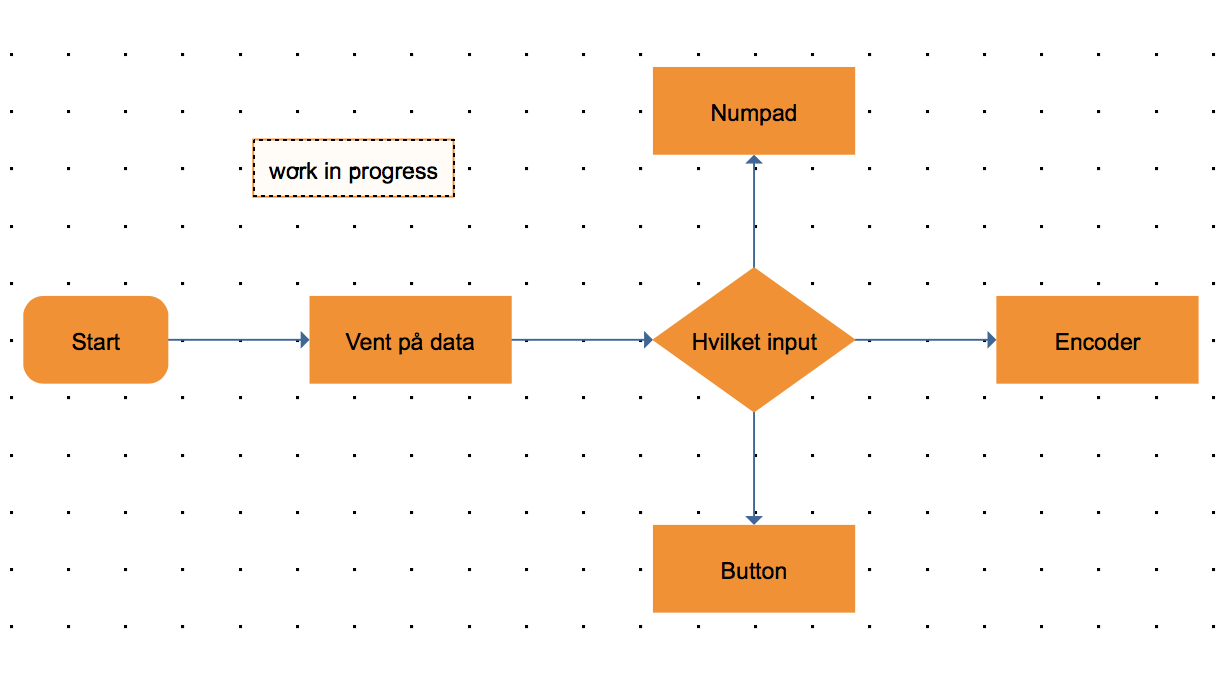
\includegraphics[width=11cm]{billeder/ui_flowchart}
	\caption{Menusystemets opbygning beskrevet med et flowchart. [WIP!!]}
\end{figure}

Menusystemet sørger for at "lytte" efter eventuelt indkommende data, og skal, når der er data tilgængeligt, behandle den derefter. I denne buffer kan der være tre forskellige ting som har indflydelse på hvad der skal ske. Der er på "EMP-board"'et en numpad, dedikerede knapper, og en encoder. 